% ** Cuidado: El indice se actualiza al compilar 2 veces. **

% -- Configuración --
\documentclass[10pt, a4paper]{article}
\usepackage[paper=a4paper, left=1.5cm, right=1.5cm, bottom=1.5cm, top=1.5cm]{geometry}
\usepackage[utf8]{inputenc}
\usepackage[spanish]{babel}
\usepackage{float}
\usepackage{mdframed}
\usepackage[section]{placeins}
% \usepackage[colorlinks=true, linkcolor=blue]{hyperref}
\usepackage{graphicx}
\usepackage{titling}
\usepackage{verbatim}
\usepackage{minted}
\usepackage{tikz}
\usepackage{dsfont}
\usepackage{amsmath}
\usetikzlibrary{chains,fit,shapes}
\newcommand{\ig}[1]{\includegraphics[width=\textwidth]{#1}}
\newcommand{\RNum}[1]{\uppercase\expandafter{\romannumeral #1\relax}}
\usepackage{parskip}
\usepackage{handy}
\usepackage{mdframed}

 
% -- Documento --
\begin{document}

\setlength{\parindent}{25pt}

	% -- Carátula --
	
	\thispagestyle{empty}
	\title{%
	\huge{Organización del Computador \RNum{2}}\\
	\vspace{4mm}
	\large{Trabajo Práctico 3}
	}
	\date{\vspace{5mm}$2^{\mathrm{do}}$ cuatrimestre de 2013}

	\author{
		\\
		{\rm Emilio Almansi }\\
		\small{ealmansi@gmail.com}
		\and
		\\
		{\rm Álvaro Machicado }\\
		\small{rednaxela.007@hotmail.com}
		\and
		\\
		{\rm Miguel Duarte}\\
		\small{miguelfeliped@gmail.com}
	} % end author
	\maketitle

	\vspace{10mm}

	% -- Indice --

	\tableofcontents

	\clearpage
	% -- Contenido --
	% Se edita cada seccion por separado, no hay que cambiar nada acá.
	\section{Introducción}
		
Se desarrolló un kernel elemental para la arquitectura Intel x86 con soporte básico para las unidades de segmentación y paginación, manejo de interrupciones y cambio automático de tareas por hardware.

El alcance del trabajo incluye múltiples etapas del proceso de arranque de todo sistema operativo, permitiendo apreciar las herramientas que provee el procesador para la administración del sistema. Durante la etapa de incialización, es necesario llevar a cabo distintos pasos como el traspaso de modo real a modo protegido, la habilitación de la unidad de paginación, o el armado de múltiples estructuras requeridas por el procesador para el manejo de interrupciones o de tareas.

Adicionalmente, se implementó un scheduler rudimentario permitiendo realizar la ejecución por tiempo compartido de múltiples tareas definidas al tiempo de compilación, realizando un ciclo de ejecución no lineal guiado por tics del reloj.

	\clearpage

	\section{Modo real y modo protegido}
			LA GDT (\textit{Global Descriptor Table})  es una estructura de datos
que la arquitectura intel x86 utiliza para almacenar distintos descriptores
de sistema. En este trabajo sólo utilizamos 3 tipos de descriptores: El
primero y mas trivial es un descriptor nulo. El procesador produce
una excepción automáticamente cunado se intenta acceder a la posición cero
de la GDT. De esta manera el primer espacio de la tabla se rellena con
un descriptor nulo para evitar confusiones. Es decir que este descriptor
en realidad cumple una función accesoria, no modifica en nada el funcionamiento
del sistema. Sin embargo es muy cómodo que este ahí. El segundo tipo
de descriptor le corresponde a los descriptores de segmento. Los mismos
delimentan el tamaño y la ubicación de los segmentos, así como sus propiedades
(quién los puede acceder, que clase código hay adentro, etc, etc. Por último
se utilizaron descriptores de TSS para realizar el salto automático de tareas
(sobre esto vamos a hablar mas adelante con mayor profundidad, ahora sólo
se explicará la parte que concierne específicamente a la GDT).

\subsection{Segmentación flat}

	Como indica el enunciado todo el trabajo funciona con segmentación flat.
Esto significa dejar de lado la protección por segmentación armando 4 segmentos
que ocupen toda la memoria superpuestos entre si. Estos 4 segmentos son 2
con nivel de privilegio cero (máximo nivel de provilegios) y 2 con nivel de privilegio
3 (mínimo nivel de privilegios), y para cada nivel un segmento de código y uno
de datos.

	Por supuesto que esta práctica acarrea problemas, algunos de ellos graves
como por ejemplo que se pierde toda la protección por hardware brindada
por la segmentación. La contracara de esto es que se obtiene un entorno
mucho mas amistoso para programar, y la mayoría de la seguridad que se pierde
por la segmentación se puede recuperar utilizando de manera adecuado la paginación.

\subsection{Descriptores de segmento}

	Los descriptores de segmento se hardcodean en tiempo de compilación. Es decir
que en el mismo código la GDT ya contiene sus descriptores de segmento con
los parámetros adecuados. Es importante que esto se puede realizar exclusivamente
porque todos lo necesario para completar esos descriptores se conoce de antemano.
Esto en parte es una consecuencia de la segmentación flat.

	Una vez que el programa empieza a correr estos descriptores de segmento
no se vuelven a modificar. Se trabaja siempre los segmentos flat, por lo que no
hace falta modificar ni agregar nada. Quedan estáticos para siempre.

	Además de los segmentos flat se crea un segmento que contiene la memoria de video.
Este segmento se utilizó con fines didácticos en un principio, pero luego
todas las funciones de video que se utilizan a lo largo del trabajo acceden
a la memoria de video por medio del segmento flat de datos de nivel 0.

\subsection{Descriptores de TSS}

	Para los descriptores de TSS se eligió otra dinámica. Las TSS se encuentran
ubicadas en un arreglo de TSS que se crea dinámicamente en tiempo de ejecución, por lo
que en el momento de la compilación no se sabe el lugar donde va a estar y por lo tanto
no se puede hardcodear esa dirección.

	Lo que se hizo, entonces, fue agregar los descriptores de TSSde manera dinámica en tiempo
de ejecución. Para esto se crearon 4 funciones en C:

\begin{minted}{c}
	void tss_inicializar_entrada_gdt_tarea_inicial();
	void tss_inicializar_entrada_gdt_idle();
	void tss_inicializar_entrada_gdt_navio(unsigned int nro_tarea);
	void tss_inicializar_entrada_gdt_bandera(unsigned int nro_tarea);
\end{minted}

	Si bien estas funciones tienen mucho en común se las creo por separado
por una cuestión pragmática que sirvió para encontrar errores y \textit{bugs} mas
fácilmente.

	Estas funciones a su vez se engloban todas en otra función escrita en c que
inicializa todas las tss y se llama desde \textbf{kernel.asm}


\begin{minted}{c}
	void tss_inicializar();
\end{minted}





	
\begin{comment}
	
	En la GDT hay que poner los descriptores de segmento
y los descriptores de TSS para cada cada tarea y para cada bandera.

	La misma está representada como un arreglo ``$gdt\_entry$'' declarado
de manera global en C. Las $gdt\_entry$ son structs de 4 bytes que poseen un campo
cara cada atributo de una entrada de gdt.

	Los descriptores de segmento fueron cargados de manera estática
en tiempo de compilación. Lo mismo con el descriptor de la IDT. Esto
fue posible porque se conocen de antemano todos los valores
necesarios para completar los descriptores.

	A la hora de cargar los descriptores de TSS nos encontramos con la
siguiente dificultad: Los descriptores de TSS fueron declarados como una
variable global en código C. Por lo tanto en tiempo de compilación
no se sabe en que dirección van a ser cargados. Por este motivo se cargan
de manera dinámica mediante una función que se llama desde kernel.asm. La
función sencillamente crea una entrada más en el arreglo que representa 
de $gdt\_entry$ con los atributos adecuados.
\end{comment}

	\clearpage

	\section{Global Descriptor Table (GDT)}
			LA GDT (\textit{Global Descriptor Table})  es una estructura de datos
que la arquitectura intel x86 utiliza para almacenar distintos descriptores
de sistema. En este trabajo sólo utilizamos 3 tipos de descriptores: El
primero y mas trivial es un descriptor nulo. El procesador produce
una excepción automáticamente cunado se intenta acceder a la posición cero
de la GDT. De esta manera el primer espacio de la tabla se rellena con
un descriptor nulo para evitar confusiones. Es decir que este descriptor
en realidad cumple una función accesoria, no modifica en nada el funcionamiento
del sistema. Sin embargo es muy cómodo que este ahí. El segundo tipo
de descriptor le corresponde a los descriptores de segmento. Los mismos
delimentan el tamaño y la ubicación de los segmentos, así como sus propiedades
(quién los puede acceder, que clase código hay adentro, etc, etc. Por último
se utilizaron descriptores de TSS para realizar el salto automático de tareas
(sobre esto vamos a hablar mas adelante con mayor profundidad, ahora sólo
se explicará la parte que concierne específicamente a la GDT).

\subsection{Segmentación flat}

	Como indica el enunciado todo el trabajo funciona con segmentación flat.
Esto significa dejar de lado la protección por segmentación armando 4 segmentos
que ocupen toda la memoria superpuestos entre si. Estos 4 segmentos son 2
con nivel de privilegio cero (máximo nivel de provilegios) y 2 con nivel de privilegio
3 (mínimo nivel de privilegios), y para cada nivel un segmento de código y uno
de datos.

	Por supuesto que esta práctica acarrea problemas, algunos de ellos graves
como por ejemplo que se pierde toda la protección por hardware brindada
por la segmentación. La contracara de esto es que se obtiene un entorno
mucho mas amistoso para programar, y la mayoría de la seguridad que se pierde
por la segmentación se puede recuperar utilizando de manera adecuado la paginación.

\subsection{Descriptores de segmento}

	Los descriptores de segmento se hardcodean en tiempo de compilación. Es decir
que en el mismo código la GDT ya contiene sus descriptores de segmento con
los parámetros adecuados. Es importante que esto se puede realizar exclusivamente
porque todos lo necesario para completar esos descriptores se conoce de antemano.
Esto en parte es una consecuencia de la segmentación flat.

	Una vez que el programa empieza a correr estos descriptores de segmento
no se vuelven a modificar. Se trabaja siempre los segmentos flat, por lo que no
hace falta modificar ni agregar nada. Quedan estáticos para siempre.

	Además de los segmentos flat se crea un segmento que contiene la memoria de video.
Este segmento se utilizó con fines didácticos en un principio, pero luego
todas las funciones de video que se utilizan a lo largo del trabajo acceden
a la memoria de video por medio del segmento flat de datos de nivel 0.

\subsection{Descriptores de TSS}

	Para los descriptores de TSS se eligió otra dinámica. Las TSS se encuentran
ubicadas en un arreglo de TSS que se crea dinámicamente en tiempo de ejecución, por lo
que en el momento de la compilación no se sabe el lugar donde va a estar y por lo tanto
no se puede hardcodear esa dirección.

	Lo que se hizo, entonces, fue agregar los descriptores de TSSde manera dinámica en tiempo
de ejecución. Para esto se crearon 4 funciones en C:

\begin{minted}{c}
	void tss_inicializar_entrada_gdt_tarea_inicial();
	void tss_inicializar_entrada_gdt_idle();
	void tss_inicializar_entrada_gdt_navio(unsigned int nro_tarea);
	void tss_inicializar_entrada_gdt_bandera(unsigned int nro_tarea);
\end{minted}

	Si bien estas funciones tienen mucho en común se las creo por separado
por una cuestión pragmática que sirvió para encontrar errores y \textit{bugs} mas
fácilmente.

	Estas funciones a su vez se engloban todas en otra función escrita en c que
inicializa todas las tss y se llama desde \textbf{kernel.asm}


\begin{minted}{c}
	void tss_inicializar();
\end{minted}





	
\begin{comment}
	
	En la GDT hay que poner los descriptores de segmento
y los descriptores de TSS para cada cada tarea y para cada bandera.

	La misma está representada como un arreglo ``$gdt\_entry$'' declarado
de manera global en C. Las $gdt\_entry$ son structs de 4 bytes que poseen un campo
cara cada atributo de una entrada de gdt.

	Los descriptores de segmento fueron cargados de manera estática
en tiempo de compilación. Lo mismo con el descriptor de la IDT. Esto
fue posible porque se conocen de antemano todos los valores
necesarios para completar los descriptores.

	A la hora de cargar los descriptores de TSS nos encontramos con la
siguiente dificultad: Los descriptores de TSS fueron declarados como una
variable global en código C. Por lo tanto en tiempo de compilación
no se sabe en que dirección van a ser cargados. Por este motivo se cargan
de manera dinámica mediante una función que se llama desde kernel.asm. La
función sencillamente crea una entrada más en el arreglo que representa 
de $gdt\_entry$ con los atributos adecuados.
\end{comment}

	\clearpage

	\section{Paginación}
			La paginación es un método de direccionamiento de memoria
en el cuál se redirigen bloques de direcciones "virtuales"
a bloques de direcciones físicas. Estos bloques se llaman páginas, y
en la arquitectura intel en el modo usado en el trabajo tiene
un tamaño de 4kb (\texttt{0x1000}). La gran ventaja de la paginación
es que la unidad en la que se trabaja la memoria (la \textit{página})
tiene siempre el mismo tamaño, lo cuál hace que sea fácil hacer manejos
complejos de memoria.

	En la arquitectura intel x86 la paginación se maneja mediante
una estructura de sistema en memoria en 2 niveles. El primer nivel se llama
\textit{page directory} y el segundo \textit{page table}. Los page directory
contienen las direcciones donde se ubican los page table y los page
table contiene direcciones físicas de páginas. De esta manera una dirección
virtual (es decir la dirección a la que accede una tarea) se interpreta
como un índice en el page directory, un índice en la page table obtenida y
, finalmente, un offset para la página encontrada en el page table.

	La siguiente gran ventaja de todo esto es que uno puede tener muchas
estructuras de paginación en memoria y asignarle una distinta a cada tarea.
Esto se hace mediante un registro de control, el \textbf{cr3}. Cuando la
paginación está activa cada vez que se realiza un acceso a memoria
el procesador usa el cr3 para encontrar la dirección del page dir. Modificando
el valor de cr3 se puede hacer que diferentes tareas tengan diferentes \textit{mapas de memoria}
, es decir que cuando accedan a iguales direcciones virtuales lleguen a
diferentes direcciones físicas.

	Si bien mas adelante se va a hablar sobre la seguridad
de manera específica es importante mencionar que debido a que la
segmentación flat detruye todos los sistemas de seguridad que provee
la segmentación la paginación se debe tratar con mucho cuidado, pues
este mecanismo tiene que asegurar toda la seguridad y la integridad de la memoria.

	Además el mapeo de páginas tiene que permitir que las tareas
se ejecuten como si su código estuviera en la posición 1GB (\texttt{0x40000000})
y puedan leer (pero no escribir) desde las direcciones \texttt{0x40002000-0x40002FFF}
direcciones de memoria del kernel.

	Para lograr todo esto implementamos un esquema de paginación en el cuál
existen páginas compartidas y páginas privadas. Pero además existen tablas
de páginas compartidas y tablas de páginas privadas. Además se tuvo especial
cuidado con los permisos otorgados a cada tabla para evitar accesos a memoria
indeseados.

\subsection{Implementación del mapa de memoria.}
	El mapa de memoria se inmplementó tal cuál lo dice el enunciado. Hay
identity mapping en los primeros 8mb y después cada tarea tiene
los mapeos que necesita para acceder a su código y al ancla.
	
	En tiempo de ejecución se generan todas las estructuras necesarias
para que el sistema y las tareas puedan funcionar. Esto incluye un page directory para cada
tarea, 1 para el kernel, 1 page table privado de cada tarea (con
permisos de usuario) y 2 page table compartidos(con permisos de administrador).

	Las page table privadas en un principio se inicializan en cero, luego
se actualizan de manera adecuada con funciones de mapeo de página
de las que se hablará mas adelante.

	La otra acción que se realiza en este momento es la de
copiar el código de las tareas de la tierra al mar. Elegimos hacerlo
en este momento porque así ya se pueden hacer los mapeos y dejar
todo todo listo para el momento en que empicen a correr las tareas.

	Todo explicado recién se hacer mediante una sola función escrita en c
que luego se llama desde kernel. asm
\newpage
	Los page table compartidos tienen los mapeos de las direcciones del kernel.
Esas direcciones estar mapeadas en todas las tareas y con los mismos atributos, motivo
por le cuál decidimos hacerlos comunes. Esto significa todas las primeras entradas
de page dir apuntan al mismo page table, el cuál redirecciona con permisos de administrador
a los primeros 4mb de kernel, del mismo modo todas las segundas entradas
de page dir apuntan también a una page table común que direcciona
a la segunda parte del kernel.


\begin{figure}[h]
\begin{center}
  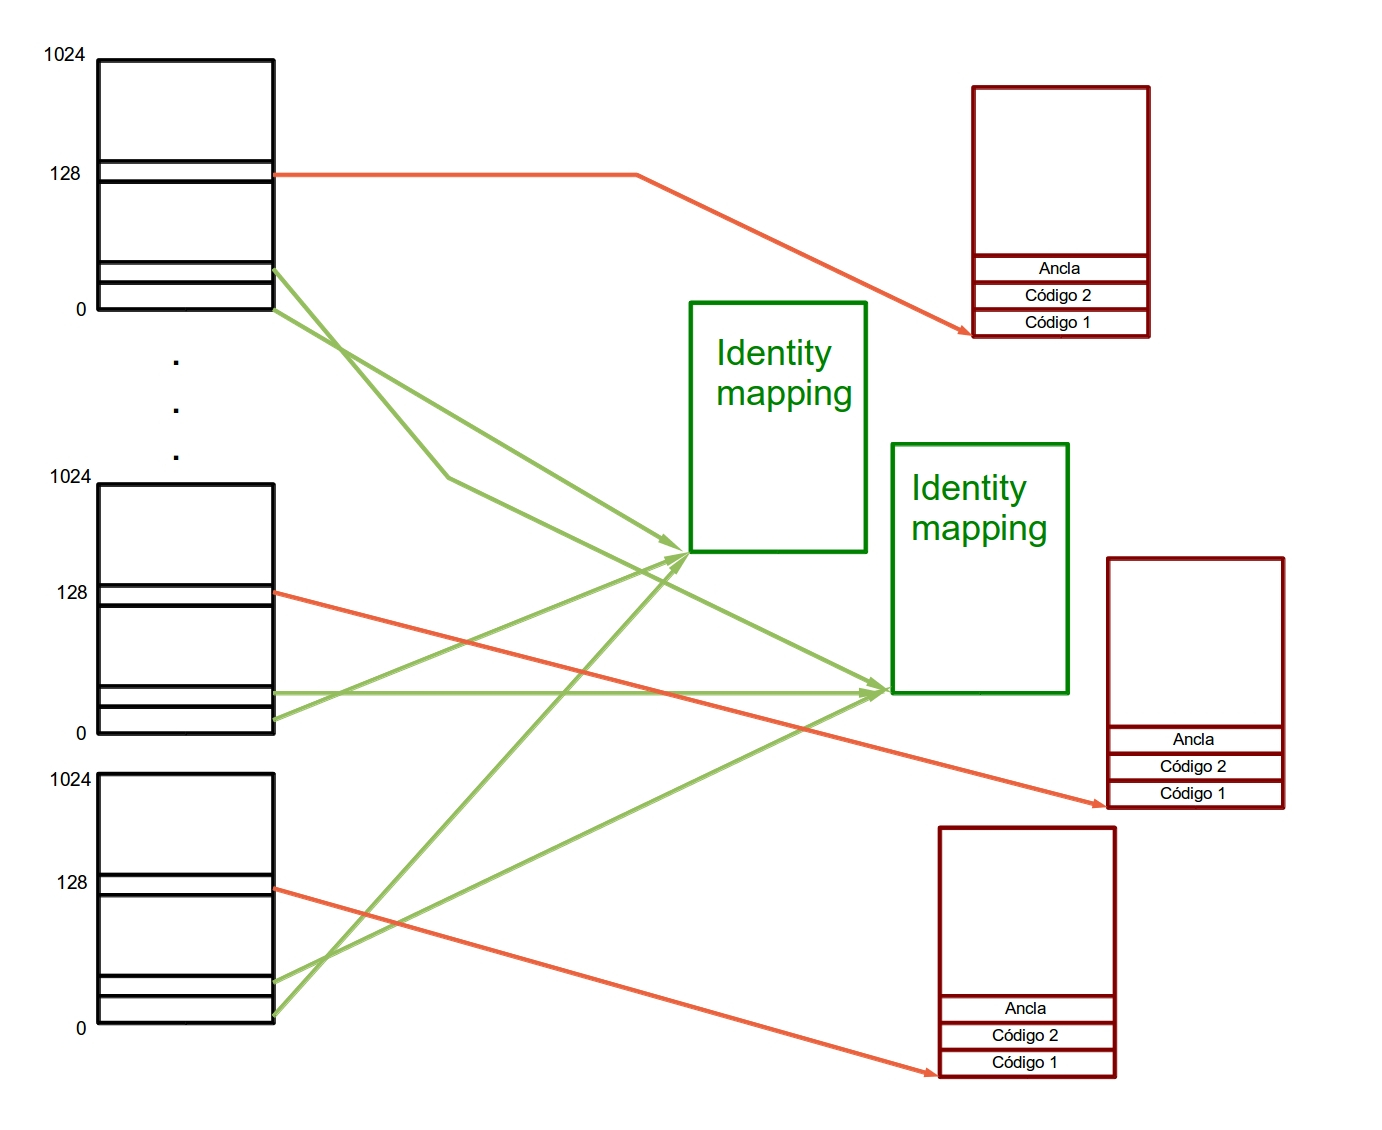
\includegraphics[scale=0.3]{secciones/dibujitos/diagramapaginas.jpg}
\end{center}
\caption{Esquema de las estructuras de paginación}
\label{fig:diagramapaginas}
\end{figure}


	Una vez que el sistema está corriendo los mapeos de página se modifican
en tiempo real mediante dos funciones que se encargan de crear
mapeos de página y de borrar mapeos de página.

\begin{minted}{c}
void mmu_mapear_pagina (unsigned int virtual, unsigned int cr3, unsigned int fisica, unsigned int attr) 
void mmu_unmapear_pagina (unsigned int virtual, unsigned int cr3) 
\end{minted}


	La función encargada de deshacer los mapeos termina con realizando un flush
de la tlb para asegurar la coherencia de todas las estructuras de paginación (
al cambiar un mapeo puede pasar que el mapeo almacenado en la tlb no coincida
más con la realidad).

	Todo esto fue implementado en C. Tanto las funciones
encargadas de crear las estructuras como las funciones encargadas
de los mapeos. Lo único que se hace desde \textit{kernel.asm} es
llamar a esas funciones en el momento adecuado.

\subsection{Activando la paginación}

	La paginación se activa mediante el bit de paginación activa en el
registro \textbf{cr0}. Es indispensable que en el momento en que se
activa ese bit cr3 ya esté seteado de manera adecuada y al menos las
estructuras de paginación del kernel esten debidamenta cargadas en memoria.



\begin{comment}
	La parte de paginación se resolvió de manera bastante intuitiva.

	Se crearon funciones en C que se encargar de inicializar los directorios
de páginas del kernel y de las tareas. Un detalle importante de la implementación
es que tanto el kernel como las tareas comparten las primeras 2 tablas de páginas
de sus directores de páginas.

	Estas dos tablas son las que se hacen con identity mapping. El identity mapping
está en todos los mapas de memoria de la misma manera y con los mismos atributos. Además
nunca debe ser cambiado a lo largo de la ejecución de todo el programa en ninguno de los
mapas. Por eso decidimos crear sólo 2 tablas de páginas y hacer que todas las tareas lo compartan.

	En un princio a cada tarea se le asigna una tabla extra inicializada en cero.
Luego mediante las funciones para mapear páginas se completan estas tablas de manera adecuada
para que se efectivicen los mapeos.

	Es importante notar que el resultado final de esto es que cada tarea tiene mapeadas
2 tablas con identity mapping y con proviligios restringidos (sólo para supervisor) y
luego un par de páginas mas con permisos de usuario, que son donde efectivamente va a trabajar.

	Todo eso se englobó en las siguientes funciones de C:
	
\begin{minted}[tabsize=4]{c}
	void mmu_inicializar_dir_kernel();
	void mmu_inicializar_paginas_kernel();
	void mmu_inicializar_tareas();
\end{minted}

	$mmu\_inicializar\_tareas$ no solo inicializar los directorios de páginas sino
que además hace los mapeos de páginas correspondientes.

	Finalmente esas funciones se llaman dentro de kernel.asm. Una vez terminado eso
se habilita la paginación.

\end{comment}

	\clearpage

	\section{Interrupciones}
			Las interrupciones y las excepciones son el método a través del cuál 
se logra interactuar con agentes externos, asegurar la integridad del sistema 
ante la ocurrencia de errores, o administrar los recursos del sistema. Para cada 
posible interrupción que se desea atender es necesario definir un handler de 
interrupción, o rutina de atención, y declararla a través de un descriptor
en una estructura del sistema denominada Interrupt Descriptor Table (IDT).

	En el sistema implementado se realizaron esencialmente los siguientes tipos de 
hanlders de interrupción: aquellos donde predomina la lógica con respecto 
al control de los recursos de sistema, como la interrupción generada por el reloj 
(que marca la unidad de tiempo sobre la que funciona el scheduler), la rutina de atención 
que procesa los eventos generados por el teclado, los handlers de atención a las syscalls 
(implementando servicios para las tareas del sistema), y las rutinas que proveen la lógica 
destinada a asegurar la integridad del sistema como puede ante el caso de una excepción 
como por ejemplo un Page Fault o un Segmentation Fault.

\subsection{Interrupciones de control de flujo y administración de sistema}

	
	La principal encargada de controlar el flujo de ejecución en el sistema es la int0x32: 
la interrupción generada por el reloj. Esta interrupción funciona de manera muy cercana 
al scheduler, consultándole cuál tarea es la próxima a ejecutar y realizando el cambio 
de tarea de ser necesario. El scheduler implementado tiene un valor de retorno distinguido: 
si retorna un valor igual a 0, significa que la tarea ejecutándose actualmente debe seguir haciéndolo, 
si por el contrario devuelve cualquier otro número se lo interpreta como un índice en
la GDT al que se debe realizar un \texttt{jmp far}, suscitando un cambio de contexto 
automático.

	Por otra parte, antes de realizar el \texttt{jmp far} es importante
verificar si la tarea a la que se va a saltar es una bandera o un
navío. Antes de saltar a una bandera, se reinicializa su TSS para
que el EIP vuelva a apuntar al comienzo de la función. Si esto no se hiciera, 
la ejecución seguiría a partir de la interrupción de fin de bandera
y ese no es el compartamiento esperado. En los navíos, en cambio, sí se espera
que la ejecución continúe donde fue interrumpida.

	Es importante contemplar el hecho de que cuando se retoma la ejecución de una tarea, 
su EIP va a estar ubicado adentro de la interrupción donde se detuvo, por lo tanto tiene 
que siempre haber un JMP al final del llamado, incluso luego de un \texttt{jmp far}.
	
	Por último todos los handlers referidos a las excepciones de
sistema (page fault, etc) al final también cambian el flujo de ejecución
pues luego de la lógica referida a la seguridad tienen que retomar
el flujo de ejecución a algún lado, ya sea al lugar donde vino o
, en caso de que esa tarea haya sido desalojada, a algún otro lado
(la tarea idle).

\subsection{Interrupciones de seguridad}

	Las excepciones de sistema como \textit{General Protection}
son el mejor ejemplo. El algoritmo de estas interrupciones es
sencillo, lo que hace es verificar que quién produjo
esa excepción sea efectivamente una tarea. Si fue una tarea la desaloja, 
sino Interrumpe el sistema y avisa que hubo una excepción. Luego
de desalojar la tarea sencillamente salta hacia la tarea idle. Además
todas estas interrupciones tienen exactamente la misma lógica, por lo
que en principio se podrían implementar todas con un macro de nasm.
El único código específico que implementamos para cada una es una funcion de C
que actualiza la pantalla de manera adecuada. Sobre esto se hablará
mas en detalla en la sección de pantalla.

	La syscalls también tienen que hacer algunas verificaciones de
seguridad. Las banderas no pueden llamar a las funciones de los barcos
y los barcos no pueden llamar a la interrupción de final de bandera.

	La interrupción de reloj debe verificar que el contexto en el
que se está ejecutando no sea el de una bandera, pues si es así
debe hacer desalojarla. 



\begin{comment}
	Las interrupciones se manejaron de 2 maneras diferentes:

	Por un lado están las excepciones de sistema. De esas sólo se busca
que si una tarea las produce esta sea desalojada. De esta manera se pudieron
implementar mediante un macro sin mayores inconvenientes.

	Por otro lado están las otras interrupciones: La de reloj, la de teclado
y las syscalls. Estas tuvieron que elaborarse de manera mas detenida.

	La interrupción de teclado basicamente es un gran $switch$ que verifica si
el contenido del código obtenido. Si este coincide con alguna de las teclas esperadas
(``e'',``m'', ``0-9'') entonces realiza la acción debida en pantalla.

	En las syscalls se tiene el cuidado de verificar quién las llama y como. Muchas
posibles llamadas a syscals son ilegales. Por ejemplo si la llamada a una int0x50 la realiza
una bandera esta debe ser desalojada. Lo mismo si esa interrupción es llamada con parámetros ilegales.
Toda esta lógica se implementó medante una función escrita en C y llamada desde assembler.

	La interrupción de reloj terminó siendo la mas compleja. Para implementarla lo que se hizo, entonces,
fue realizar una función en c que se llama desde la interrupción. Esta función verifica si quién
se estaba ejecutando al memento de la interrupción de reloj era una bandera. En ese caso la desaloja.
Luego le pide al scheduler el índice de la GDT que necesario pra realizar un JUMP far al contexto
de la otra tarea. A continuación se fija si la próxima tarea a ejecutarse es una bandera. Si es una bandera
entonces primero reinicia su tss y luego, si, realiza el jmp far.
\end{comment}
	

	\clearpage

	\section{Manejo de tareas}
			El sistema implementado ejecuta un total de hasta 19 tareas en forma itinerante: 
ocho navíos, ocho banderas y la tarea idle. Además, como se dijo previamente, 
los navíos deben comenzar a ejecutarse siempre desde el punto donde fueron interrumpidos, 
mientras que las banderas comienzan siempre desde el inicio de la función. Esto requiere 
mantener registro del estado de los navíos (es decir, guardar todo su contexto para que 
pueda retomar la ejecución sin ser alterada), y un método para intercambiar el contexto 
de diferentes tareas.

	Para resolver este requerimiento, se optó por el cambio automático 
de tareas por hardware que provee la arquitectura Intel x86. Para utilizar este mecanismo, 
es necesario mantener para cada tarea en ejecución una estructura llamada Task State 
Segment (TSS), que consiste en un espacio de memoria donde se guarda (y de donde se 
recupera) el contexto de la tarea de forma automática. Como se dijo en la sección sobre la GDT, 
cada TSS requiere también un descriptor de TSS en la tabla GDT, de forma tal que se pueda 
accionar el mecanismo mediante un \texttt{jmp far}, configurando el selector del salto 
al descriptor TSS de la tarea a la que se desea comenzar a ejecutar.

	Cada vez que se realiza un salto a una nueva tarea, el contexto actual sobreescribe 
la TSS apuntada por el registro Task Register (TR). Esta característica tuvo dos implicaciones 
en la implementación realizada. En primer lugar, previo a la ejecución de la primer tarea 
mediante este mecanismo, el contexto de ejecución no corresponde a ninguna tarea en particular, y 
no tendría sentido que sobreescriba la TSS de ninguna tarea. Por esta razón, se genera una 
TSS adicional para una \"tarea inicial\", cuyo único propósito es ser la TSS que se altera 
al realizar el primer salto. En segundo lugar, como a priori no es necesario guardar el estado de las tareas que ejecutan funciones bandera, se podría prescindir de construir una TSS para cada 
una de ellas. Sin embargo, para proveer un espacio de memoria donde escribir el contexto actual 
cada vez que se interrumpe una tarea tipo bandera, se optó por brindar una TSS a cada una de ellas.

	Para mantener el comportamiento acíclico de las tareas bandera, en vez de recuperar el 
contexto de su TSS asociada (allí se encuentra el estado de la última vez que se ejecutó), se
reinicializa la TSS al igual que la primera vez que fue ejecutada, garantizando que siempre se
procesa desde el comienzo.	

	\clearpage


	\section{Protección}
			Las tareas corren en el anillo de seguridad 3. El kernel en anillo 0.
A nivel paginación las tareas son usuario y el kernel es supervisor.

	Las tareas no pueden acceder a memoria del kernel bajo ninguna circinstancia.
Esto está asegurado en el mapa de memoria. El mismo si bien incluye las tablasde memoria
del kernel las incluye con un privilegios mayor, por lo tanto si una tarea intenta
acceder a esas páginas cae un page fault que termina en el desalojo de esa tarea.

	El kernel está programado para no tener que incurrir en ninguna excepción especial,
lo tanto el código que se ejecuta cuando ocurre una excepción es siempre el mismo. Desalojar
a esa tarea y saltar a la tarea iddle. Esto asegura que toda tarea que realice una acción
ilegal que produzca uan excepción (dividir entre cero, seg fault, page fault, etc) será
desalojada.

	Además hay un par de cuestiones extra. Por ejemplo, una bandera no puede llamar a una int0x50.
Si hace esto inmediatamente es desalojada.

	\clearpage

	\section{Scheduler}
		
Dadas las dieciséis tareas del sistema -ocho navíos, ocho banderas-, el scheduler desarrollado ejecuta todas las tareas de forma itinerante, alternando entre ellas de la siguiente forma: se dedican tres ticks de reloj a ejecutar navíos, se procesan todas las funciones bandera pertenecientes a navíos activos, y luego se retoma la ejecución de los navíos. Los navíos se ejecutan secuencialmente por lo que todos reciben la misma cantidad de ticks mientras no sean desalojados.

Para implementar esta lógica, se realizaron colas circulares basadas en arreglos para los índices de la tabla GDT de los navíos y las banderas\footnote{De los descriptores de sus tablas TSS, para ser preciso.}. Como no se ingresan nuevos elementos dinámicamente, el mecanismo de elminación de una tarea se puede realizar sencillamente marcando su entrada con un valor inválido, como el 0 ya que nunca es un índice válido en la tabla.

Para mantener el orden de ejecución descripto, se guardaron adicionalmente contadores para la cantidad de navíos activos en la cola, la cantidad de navíos pendientes hasta alternar con la ejecución de banderas, e inversamente la cantidad de banderas pendientes.

De esta forma, se mantiene el invariante de que al menos uno de los dos contadores de tareas pendientes es nulo, y se consumen elementos de la cola opuesta hasta terminar la ronda. Es decir, inicializando la cantidad de navíos pendientes a 3 y la cantidad de banderas pendientes a 0, se dedicarán 3 ticks a ejecutar navíos, y luego se asigna la cantidad de tareas activas al contador de banderas pendientes, asegurando que se llamen todas las banderas disponibles.

Como ya se dijo, cuando una tarea necesita ser desalojada, su entrada correspondiente y la de su navío o bandera asociada se anulan, permitiendo evitar su ejecución simplmente salteando los ceros que se encuentren en la cola.

Finalmente, en el caso de que hayan sido desalojadas todas las tareas, el scheduler retorna un valor distinguido igual a 0, procediendo a ejecutarse la tarea idle initerrumpidamente de allí en adelante.
	\clearpage

	\section{Conclusiones}
			A lo largo de todo el trabajo se presentó la enorme cantidad de inconvenientes
que conlleva trabajar sobre la nada. Para realizar el trabajo fue imprecindible entender
lo que estaba sucediendo en el kernel a muy bajo nivel, pues constanemente surgen inconvenientes
cuya explicación no suele ser evidente.

	También una cosa que se presentó es que la dificultad de la implementación asciende al infinito
si uno lo permite. En todo momento se presentan ecrucijadas sobre como realizar algo específico teniendo
una libertad casi absoluta al tener permisos de kernel. En general en esos momentos intentamos optar
por la implementación mas clara con una lógica mas sólida perdiendo en algunos casos algo de performance.
Sin embargo lo que se ganó con eso fue un código mucho mas manejable.





\end{document}
